\scanpage{3}
% The isolated pencil 2 at the foot is treated as an archive sheet number.

\diagram{\resizebox{\linewidth}{!}{{\small\setlength{\arraycolsep}{3pt}
$\begin{array}{ccc|l@{\quad}l}
V_1&V_2&V_3&V_1\ \text{\unsure{borde|bords}}\ \Gamma'_2,\Gamma'_3&
\Gamma'_1\ \text{bordé par}\ V_2,V_3\\
\overset{\deleted{\unsure{\circ|\bullet}}}{\Gamma}''_1&
\overset{\deleted{\circ}}{\Gamma}''_2&
\overset{\deleted{\circ}}{\Gamma}''_3&
V_2\ \text{borde}\ \Gamma'_3,\Gamma'_1&\Gamma'_2\ \text{---}\ V_3,V_1\\
\shortparallel&\shortparallel&\shortparallel&&\\[-.4ex]
\Gamma'_1-\partial&\Gamma'_2-\partial&\Gamma'_3-\partial&
V_3\ \text{borde}\ \Gamma'_1,\Gamma'_2&\Gamma'_3\ \text{---}\ V_1,V_2
\end{array}$}}}

\noindent\begin{minipage}[t]{.35\linewidth}
\[
\partial=\{\unsure{x},y\}
\]
\end{minipage}

\[
\begin{aligned}
\Gamma_1&=\Gamma_2\cup\Gamma_3=\Gamma'_{\unsure{2|1}}\cup\Gamma'_3
=\Gamma''_1\cup\Gamma''_2\cup\partial\\
\Gamma_2&=\Gamma_3\cup\Gamma_1=\Gamma'_3\cup\Gamma'_1
=\Gamma''_3\cup\Gamma''_1\cup\unsure{\partial|\dot\partial}\\
\Gamma_3&=\Gamma_1\cup\Gamma_2=\Gamma'_1\cup\Gamma'_2
=\Gamma''_1\cup\Gamma''_2\cup\partial
\end{aligned}
\]

\noindent\begin{minipage}[c]{.34\linewidth}
% The drawing and its labels retain their quarter-turned position on the sheet.
% Small retraced spurs on the outline are drawn as strokes, not interpreted as arrows.
\figure{\resizebox{\linewidth}{!}{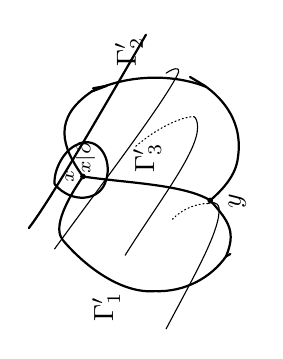
\begin{tikzpicture}[x=.8cm,y=.8cm,line cap=round,line join=round]
\begin{scope}[rotate=90]
\draw[thick] (0,2.02) .. controls (-.48,2.35) and (-.84,2.48) .. (-1.01,2.34)
 .. controls (-1.47,1.95) and (-1.86,1.38) .. (-1.82,.88)
 .. controls (-1.84,.40) and (-1.60,-.02) .. (-1.27,-.25)
 .. controls (-.89,-.41) and (-.72,-.31) .. (-.38,0);
\draw[thick] (0,2.02) .. controls (.47,2.36) and (.92,2.51) .. (1.35,1.88)
 .. controls (1.67,1.19) and (1.59,.47) .. (1.42,.06)
 .. controls (1.14,-.32) and (.75,-.51) .. (.30,-.44)
 .. controls (.03,-.41) and (-.19,-.22) .. (-.38,0);
\draw[thick] (0,2.02) .. controls (-.10,1.38) and (-.12,.42) .. (-.38,0);
\draw[thick] (-.12,2.47) .. controls (.10,2.49) and (.43,2.32) .. (.51,2.10)
 .. controls (.66,1.78) and (.28,1.55) .. (-.05,1.65)
 .. controls (-.41,1.74) and (-.43,2.22) .. (-.12,2.47);
\draw[thick] (1.35,1.88) -- (1.44,1.64) -- (1.40,1.86);
\draw[thick] (1.43,.07) -- (1.58,.32);
\draw[thick] (-1.27,-.25) -- (-1.23,-.32);
\draw[thick] (-.82,2.88) .. controls (-.40,2.55) and (1.18,1.64) .. (2.25,1.02);
\draw (-.82,2.88) -- (-.27,2.50);
\draw (-1.15,2.47) .. controls (-.25,1.82) and (1.25,.67) .. (1.66,.50)
 .. controls (1.75,.48) and (1.71,.60) .. (1.64,.70);
\draw (-1.25,1.35) .. controls (-.42,.83) and (.38,.20) .. (.78,.20)
 .. controls (.88,.20) and (.94,.23) .. (.95,.26);
\draw (-2.42,.70) .. controls (-1.60,.27) and (-.85,-.17) .. (-.50,-.14)
 .. controls (-.39,-.12) and (-.41,-.01) .. (-.43,.04);
\draw[densely dotted] (.48,1.18) .. controls (.79,.82) and (.95,.44) .. (.95,.26);
\draw[densely dotted] (-.68,.60) .. controls (-.50,.43) and (-.43,.20) .. (-.43,.04);
\fill (0,2.02) circle (.045);
\fill (-.38,0) circle (.045);
\node[rotate=90] at (-2.07,1.65) {$\Gamma'_1$};
\node[rotate=90] at (1.98,1.29) {$\Gamma'_2$};
\node[rotate=90] at (.30,1.00) {$\Gamma'_3$};
% The x-like glyph is already marked at its first occurrence in the set above.
\node[rotate=90,inner sep=0pt] at (0,2.23) {\scriptsize $x$};
\node[rotate=90,inner sep=0pt] at (.30,1.98) {\scriptsize $\deleted{\unsure{x|\partial}}$};
\node[rotate=90] at (-.40,-.43) {$y$};
\end{scope}
\end{tikzpicture}}}
\end{minipage}\hfill
\begin{minipage}[c]{.64\linewidth}
\[
\resizebox{\linewidth}{!}{$\displaystyle
\Gamma_3^{\deleted{\circ}}=\Gamma''_1\cup\Gamma''_{\unsure{2|1}}\cup\partial
\ \big|\quad U_3=V_1\cup V_2\cup\Gamma''_3\quad\big|\quad V_3$}
\]

\[
\dot U_3=\Gamma_3\qquad U_3\cup
\]
\end{minipage}

\[
\unsure{\cdot}\ U,C,V
\]
% archive sheet number: 2
